\section{Projektmanagement}
Für die Projektplanung und -verwaltung wurde auf verschiedene Hilfsmittel zurückgegriffen. Als Projektvorgehensmodell wurde in groben Zügen \gls{rup} angewendet. Zum Projektbeginn wurde ein Grobzeitplan erstellt und folgende Meilensteine definiert:

\begin{longtable}{>{\RaggedRight}r|>{\RaggedRight}p{7.3cm}|l}
& &  \\ [-1.5ex]
\textbf{\#} & \textbf{Beschreibung} & \textbf{Datum} \\ [1ex] \hline \hline & &  \\ [-1.5ex]
0 & Kickoff Meeting & 31.01.2013 \\ [1ex] \hline & &  \\ [-1.5ex]
1 & Requirements definiert & 15.03.2013 \\ [1ex] \hline & &  \\ [-1.5ex]
2 & Schnittstellen definiert & 22.03.2013 \\ [1ex] \hline & &  \\ [-1.5ex]
3 & Erster Prototyp bei der cnlab Software AG präsentiert & 28.03.2013 \\ [1ex] \hline & &  \\ [-1.5ex]
4 & Erster Feldtest Stäheli & 31.03.2013 \\ [1ex] \hline & &  \\ [-1.5ex]
5 & Zwischenpräsentation mit Gegenleser und zweiter Prototyp vorgestellt & 26.04.2013 \\ [3.5ex] \hline & &  \\ [-1.5ex]
6 & Komplettsystem Test & 02.05.2013 \\ [1ex] \hline & &  \\ [-1.5ex]
7 & Feature Freeze & 24.05.2013 \\ [1ex] \hline & &  \\ [-1.5ex]
8 & Code Freeze & 31.05.2013 \\ [1ex] \hline & &  \\ [-1.5ex]
9 & Abstract / Broschürentext einreichen &  07.06.2013 \\ [1ex] \hline & &  \\ [-1.5ex]
10 & Abgabe und Präsentation Poster & 14.06.2013 \\ [1ex] 
\caption{Übersicht aller Meilensteine}
\end{longtable} 

Die Gesamtplanung mit den An- und Abwesenheiten der Projektmitgliedern und den Meilensteinen wurde in einer Excel Datei erfasst. Diese Datei befindet sich auf der CD. Die aufgewendete Arbeitszeit zu den jeweiligen Arbeitspaketen wurde im Projektverwaltungstool Redmine aufgezeichnet und kann unter \url{http://ita.cnlab.ch/redmine/projects/ba-tourlive} eingesehen werden.
\\
\subsection{Zeitauswertung}
Abbildung \ref{fig:zeitauswertung} gibt einen Überblick in die Anzahl aufgewendeter Arbeitsstunden pro Person und Semesterwoche. Geplant wurde mit einem Projektaufwand von 1080 Stunden. Die Ist-Zeit beträgt 1326 Stunden und übersteigt die Soll-Zeit um 246 Stunden. Eine personenbezogene Zeitauswertung befindet sich auf der beiliegenden CD.

\begin{figure}[H]
	\centering
	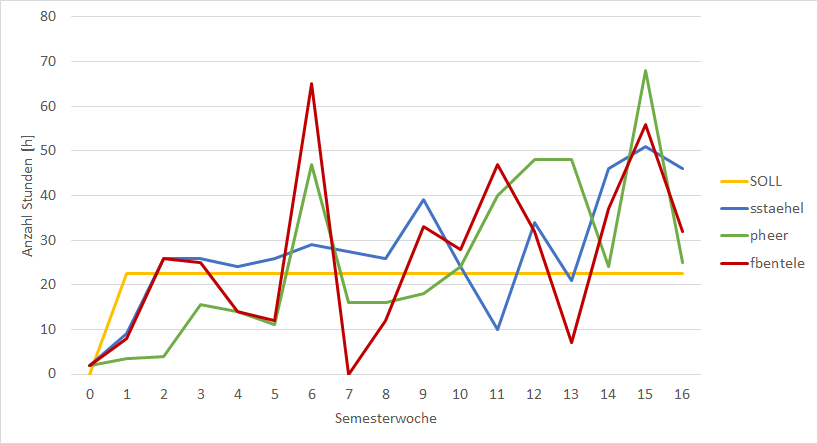
\includegraphics[width=140mm]{images/timereport.png}
	\caption{Zeitauswertung über alle Projektmitarbeiter}
	\label{fig:zeitauswertung}	
\end{figure}

\subsection{Dokumentation}
Für diese Dokumentation wurde das Textsatzprogramm {\LaTeX} verwendet. Es lässt sich optimal mit dem Versionierungssystem \textit{\gls{git}} kombinieren, was die Zusammenarbeit an der Dokumentation vereinfachte.
\\

Zu jedem Meeting mit dem Industriepartner wurde ein Protokoll geschrieben. Sämtliche Protokolle und zusätzliche Dokumente befinden sich im Word Format auf der CD.
